\section{Large Deformation Diffeomorphic Metric Mapping}
\label{sec:LDDMM}

	Of the many ways to describe variations in shapes in biology, a longstanding idea was first proposed by Thompson in his influential work \textit{"On Growth and Form"} in 1917 \cite{Thompson_1992}. Therein, he argued that variations in the shapes of biological organisms can be best described by geometrical transformations. This pioneering theory formed the basis for CA decades later with the development of computer vision and mathematical tools. In essence, CA assumes that individual shapes are described as diffeomorphic transformations of an underlying reference shape. As, in principle, an infinite number of diffeomorphisms can act on a reference shape, sets of diffeomorphisms can then be considered as an infinite dimensional manifold \cite{Marsland2020}. Accordingly, all the possible variations of a given shape can be represented within these manifolds, which are termed as 'shape spaces' \cite{Kendall1984, Monteiro2000, Rohlf2000}. These manifolds can then be enriched with Riemannian metrics which enable quantitative comparison of these shapes and further mathematical operations \cite{Younes2010, Miller2002, Miller2004}. This constitutes the basis for large deformation diffeomorphic metric mapping (LDDMM) framework \cite{Glauns2008, Durrleman2014}. Wherein, variations of anatomical shape in a population are described \textit{via} diffeomorphisms acting on an underlying reference template. These diffeomorphisms then make up the shape space, an infinite dimensional Riemannian manifold describing all possible variations of a shape in a population. The LDDMM framework can then be extended further for longitudinal shape modeling as we will discuss.  

		\subsection{Geodesics}
		
		For an initial reference shape $y_{0}$ and target shape $y_{1}$, a diffeomorphism $\phi_{1}$ exists which can be applied to transform the former to the latter (Figure \ref{fig:fig1}A). Following the convention of Bône \textit{et al.}, we denote this as $y_{1} = \phi_{1} \star y_{0}$ \cite{Bne2020}. Within the LDDMM framework, these diffeomorphisms follow the trajectories of a time-dependent vector field $t \rightarrow v_{t} \in C_{0}^{\infty} (\mathbb{R}^{d}, \mathbb{R}^{d})$ over [0,1]. Thus, starting from an identity mapping (Id), the change in $\phi_{t}$ over time ($\partial _{t} \phi_{t}$) is described as a functional composition of $v_{t}$ and $\phi_{t}$, denoted by $v_{t} \circ \phi_{t}$.(Equation \ref{eq:timevector}).
		
		\FloatBarrier
		\begin{figure}[h!]
			\centering
			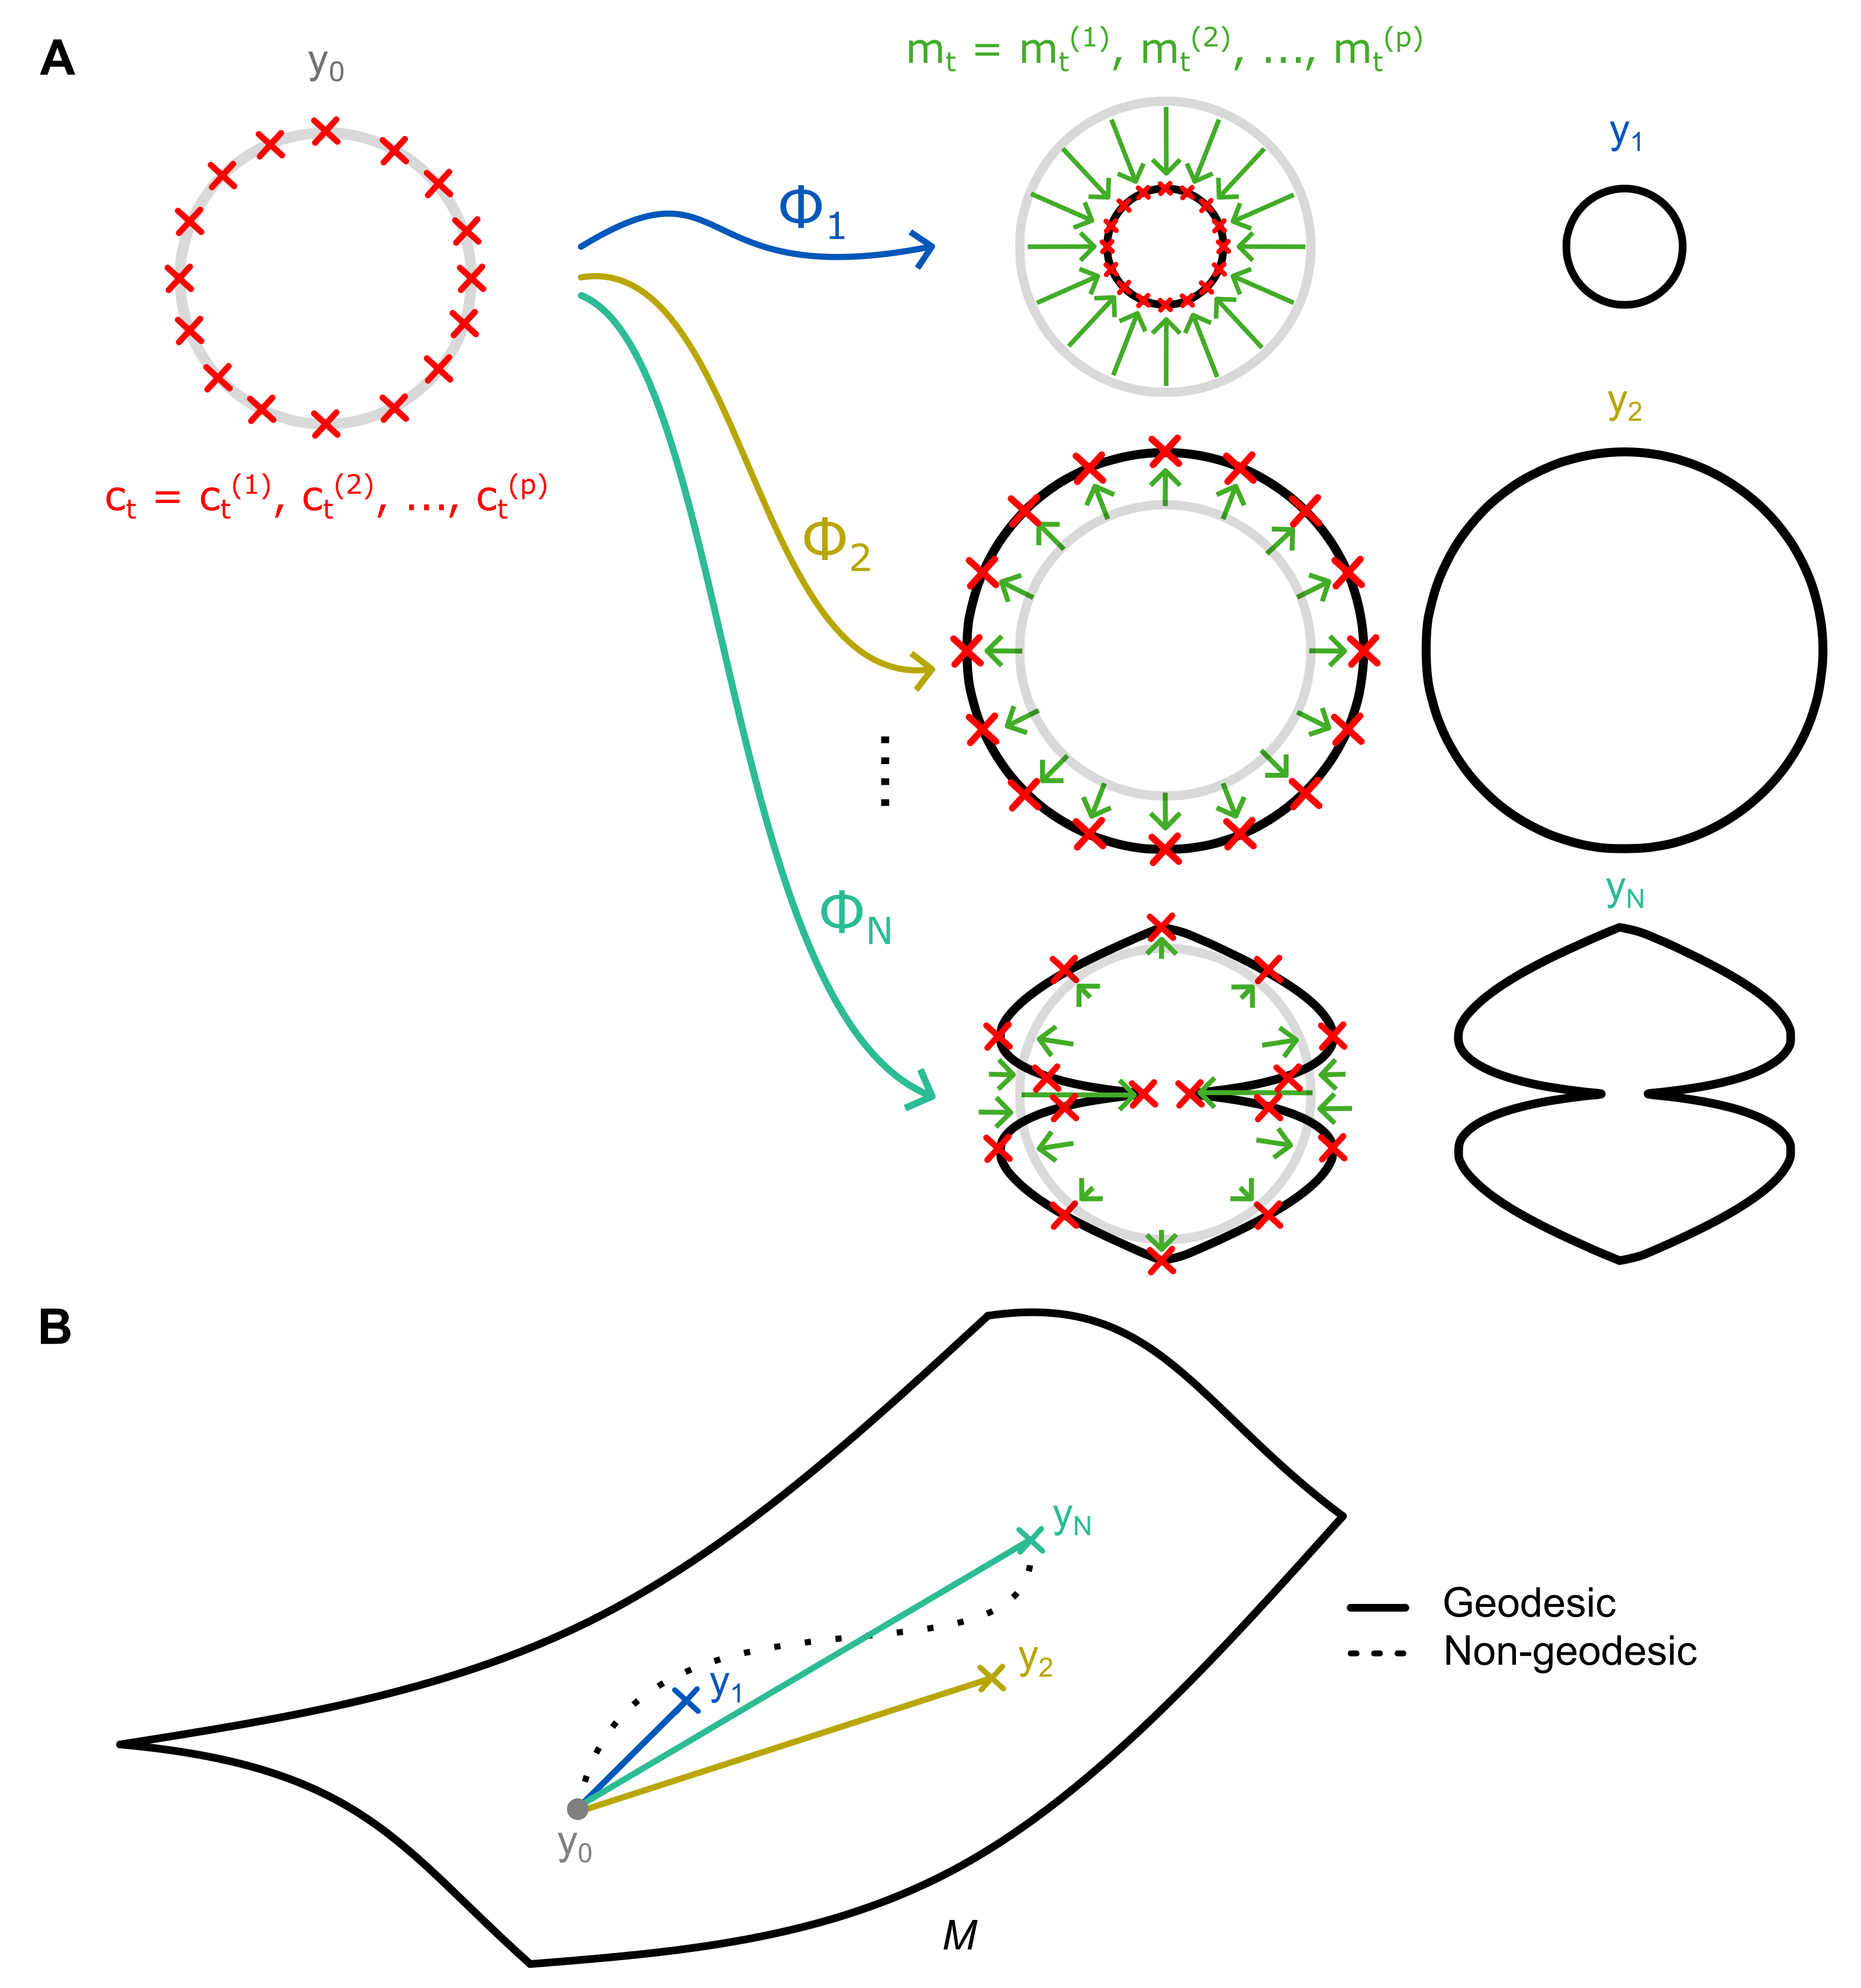
\includegraphics[scale=0.9]{fig1.png}
			\caption{\textbf{A)} An illustration of diffeomorphisms $[\phi_{1},...,\phi_{N}]$ acting on a baseline reference shape $y_{0}$ to transform it to a shape within a dataset $[y_{1},...,y_{N}]$. A diffeomorphism constitutes $p$ momentum vectors $m_{t}$ acting on a similar number of control points $c_{t}$. \textbf{B)} Diffeomorphisms within the LDDMM framework lie on a Riemannian manifold $M$. The shortest paths (\textit{i.e.,} geodesics) connecting the reference shape and other shapes are used to describe the transformation and are determined based on minimal deformational energy.}
			\label{fig:fig1}
		\end{figure}
		\FloatBarrier
		
		\begin{equation}
			\partial _{t} \phi_{t} = v_{t} \circ \phi_{t} \quad \textrm{with} \quad \phi_{0} = \textrm{Id}.
			\label{eq:timevector}
		\end{equation}

		These diffeomorphisms can be difficult to obtain and describe, especially for complex shapes and deformations. Nevertheless, Miller \textit{et al.} demonstrated that these complex deformations could be succinctly described by utilizing the principle of conservation of momentum (\textit{i.e.,} vectors of momenta) \cite{Miller2006, Vaillant2004}. Specifically, $v_{t}$ can be discretized as a Gaussian convolution $g$ of $p$ momentum vectors $m_t = m^{(1)}_{t}, . . ., m^{(p)}_{t} \in \mathbb{R}^{d}$ acting over a set of corresponding control points $c_{t} = c^{(1)}_{t},..., c^{(p)}_{t} \in \mathbb{R}^{d}$, which also influence arbitrary points $x$ (Equation \ref{eq:vecconv}, Figure \ref{fig:fig1}A). 		
		
		\begin{equation}
			v_{t} : x \in \mathbb{R}^{d} \rightarrow \sum_{k=1}^{p} g[c_{t}^{(k)}, x] \cdot m_{t}^{(k)} \in \mathbb{R}^{d}
			\label{eq:vecconv}
		\end{equation}
		
		In general notation, the Gaussian kernel function is defined as $g: x, x' \in \mathbb{R}^{d} \rightarrow \exp \vert\vert x' - x \vert\vert_{l^2}^{2} / \sigma^2$, with kernel width $\sigma > 0$. Solutions for $\phi_{t}$ are non-unique due to the infinite-dimensional nature of the underlying shape space manifold. Thus, the geodesic, that is the diffeomorphism requiring the least amount of deformational energy (Equation \ref{eq:defenergy}, Figure \ref{fig:fig1}B), is utilized \cite{Miller2002, Durrleman2014}. 
		
		\begin{equation}
			\frac{1}{2} \int_{t=0}^{1} \vert\vert v_{t} \vert\vert_{G_{c_{t}}}^{2} = \frac{1}{2} \int_{t=0}^{1} m_{t}^{T} \cdot G_{c_{t}} \cdot m_{t}
			\label{eq:defenergy}
		\end{equation}
		
		, where, $G_{c_{t}}$ is the $p \times p $ kernel symmetric positive-definite matrix of general term $g[c_{t}^{(k)}, c_{t}^{(l)}]$ and $(\cdot)^{T}$ denotes a matrix transposition. These geodesics' control points and momenta are also fully determined by their initial values and the following Hamiltonian equations (Equation \ref{eq:hamiltonian}). The former observation is particularly notable as, then, the system of initial momenta and control point locations $S_{0} = \{ c_{0}, m_{0}\}$, fully parametrize the entire flow of diffeomorphisms. 
		
		\begin{equation}
			\dot{c_{t}} = G_{c_{t}} \cdot m_{t}  \quad ; \quad \dot{m_{t}} = -\frac{1}{2} \nabla_{c_{t}} \{  m_{t}^{T} \cdot G_{c_{t}} \cdot m_{t}   \} 
			\label{eq:hamiltonian}
		\end{equation}	
		
		, where $\nabla_{c_{t}}$ is the gradient operator with respect to $c_{t}$. Thus, a Riemannian manifold $\mathscr{D}_{c_{0}}$, based on Equations \ref{eq:timevector}, \ref{eq:vecconv}, and \ref{eq:hamiltonian}, can be described as follows (Equation \ref{eq:riemanmanifold}): 
				
		\begin{equation}
			\begin{aligned}
			\mathscr{D}_{c_{t}} = \{ \phi_{1} \vert &\partial_{t}\phi_{t} = v_{t} \circ \phi_{t}, \quad \phi_{0} = \mathrm{Id}, \quad v_{t} = \mathrm{Conv}(c_{t}, m_{t}), \\
			&(\dot{c_{t}}, \dot{m_{t}}) = \mathrm{Ham} (c_{t}, m_{t}), \quad m_{0} \in \mathbb{R}^{p \times d}  \}
			\end{aligned}
			\label{eq:riemanmanifold}
		\end{equation}

		\subsection{Geodesic Regression}
			
			In representing each shape in a longitudinal dataset as a diffeomorphism of a template shape, the challenge remains in establishing the relationships between each shape. This is particularly important as deriving any underlying relationships between different shapes and independent variables (\textit{i.e.,} time) is essential for spatiotemporal shape modeling. Acquiring these relationships \textit{via} standard regression techniques, for instance, is non-trivial due to the non-Euclidean structure of the Riemannian manifolds of diffeomorphisms. Nonetheless, Fletcher proposed an extension of standard linear regression to be applicable in a manifold-based setting, termed geodesic regression \cite{fletcher2011, ThomasFletcher2012}. Their technique was then developed further for a variety of applications, but the developments of Fishbaugh \textit{et al.} for use in longitudinal shape modelling are of particular interest \cite{Fishbaugh2013, Fishbaugh2017} for our purposes. 
			
			In detail, for a longitudinal dataset of shapes with $N$ number of observations in the time range $[t_{0}, t_{N}]$, shape change over time is taken as a baseline shape $y_{0}$ being continuously deformed at each time point $t$ by a corresponding diffeomorphism $\phi_t$ (Figure \ref{fig:fig2}A). In principle, $\phi_t$ should lead to the baseline shape morphing to completely match the observed shape $y_{t} = \phi_{t} \star y_{0}$. However, in this context of estimating a holistic group-average geodesic (Figure \ref{fig:fig2}B), we note that a diffeomorphism instead leads to an estimation of the observed shape at time $t$ instead $(\hat{y_{t}} = \phi_{t} \star y_{0})$. A regression criterion can then be expressed as follows (Equation \ref{eq:shapregression}), subject to Equation \ref{eq:vecconv} and \ref{eq:hamiltonian} \cite{Fishbaugh2013, Fishbaugh2017}. 
			
			\begin{equation}
				E(y_{0}, S_{0}) = \sum_{i=1}^{N_{}} \frac{1}{2 \gamma^{2}} \vert\vert (\phi_{t_{i}} \star y_{0}) - y_{t_{i}} \vert\vert^{2} + L(S_{0})
				\label{eq:shapregression} 
			\end{equation}
			
			, where, $L(S_{0})$ represents a regularity term for the time-varying deformation, determined by the kinetic energy of the control points at $S_{0}$ (Equation \ref{eq:defenergy}). $\gamma^2$ represents a term used to balance the importance between the data and regularity terms. Thus, given a dataset of longitudinal shapes, during the minimization of Equation \ref{eq:shapregression} the baseline shape $y_{0}$, initial control point locations $c_{0}$, and initial momenta $m_{0}$ are the parameters which are estimated. This general form of geodesic shape regression was then developed further to incorporate both shape and image data based on a weighted joint optimization routine \cite{Fishbaugh2014}. Their multimodal approach demonstrated improved performances as opposed to exclusive shape or image approaches. Nevertheless, optimization schemes to solve for the underlying geodesic regressions are computationally expensive, especially for large-scale image datasets. Recently, Ding \textit{et al.} have also proposed methods to enhance their speed and effectiveness using DL \cite{Ding2019}. They demonstrated that the use of encoder-decoder networks with GPU acceleration could increase computation speeds, enabling the scaling up of studies towards larger datasets encompassing more subjects or longer timescales. Developments notwithstanding, these methods were limited to single subject regressions; geodesic regression up to this point has mainly captured spatiotemporal variability of only single subjects, thus these methods were extended further to capture populations and their intervariabilities. 

			\begin{figure}[h!]
				\centering
				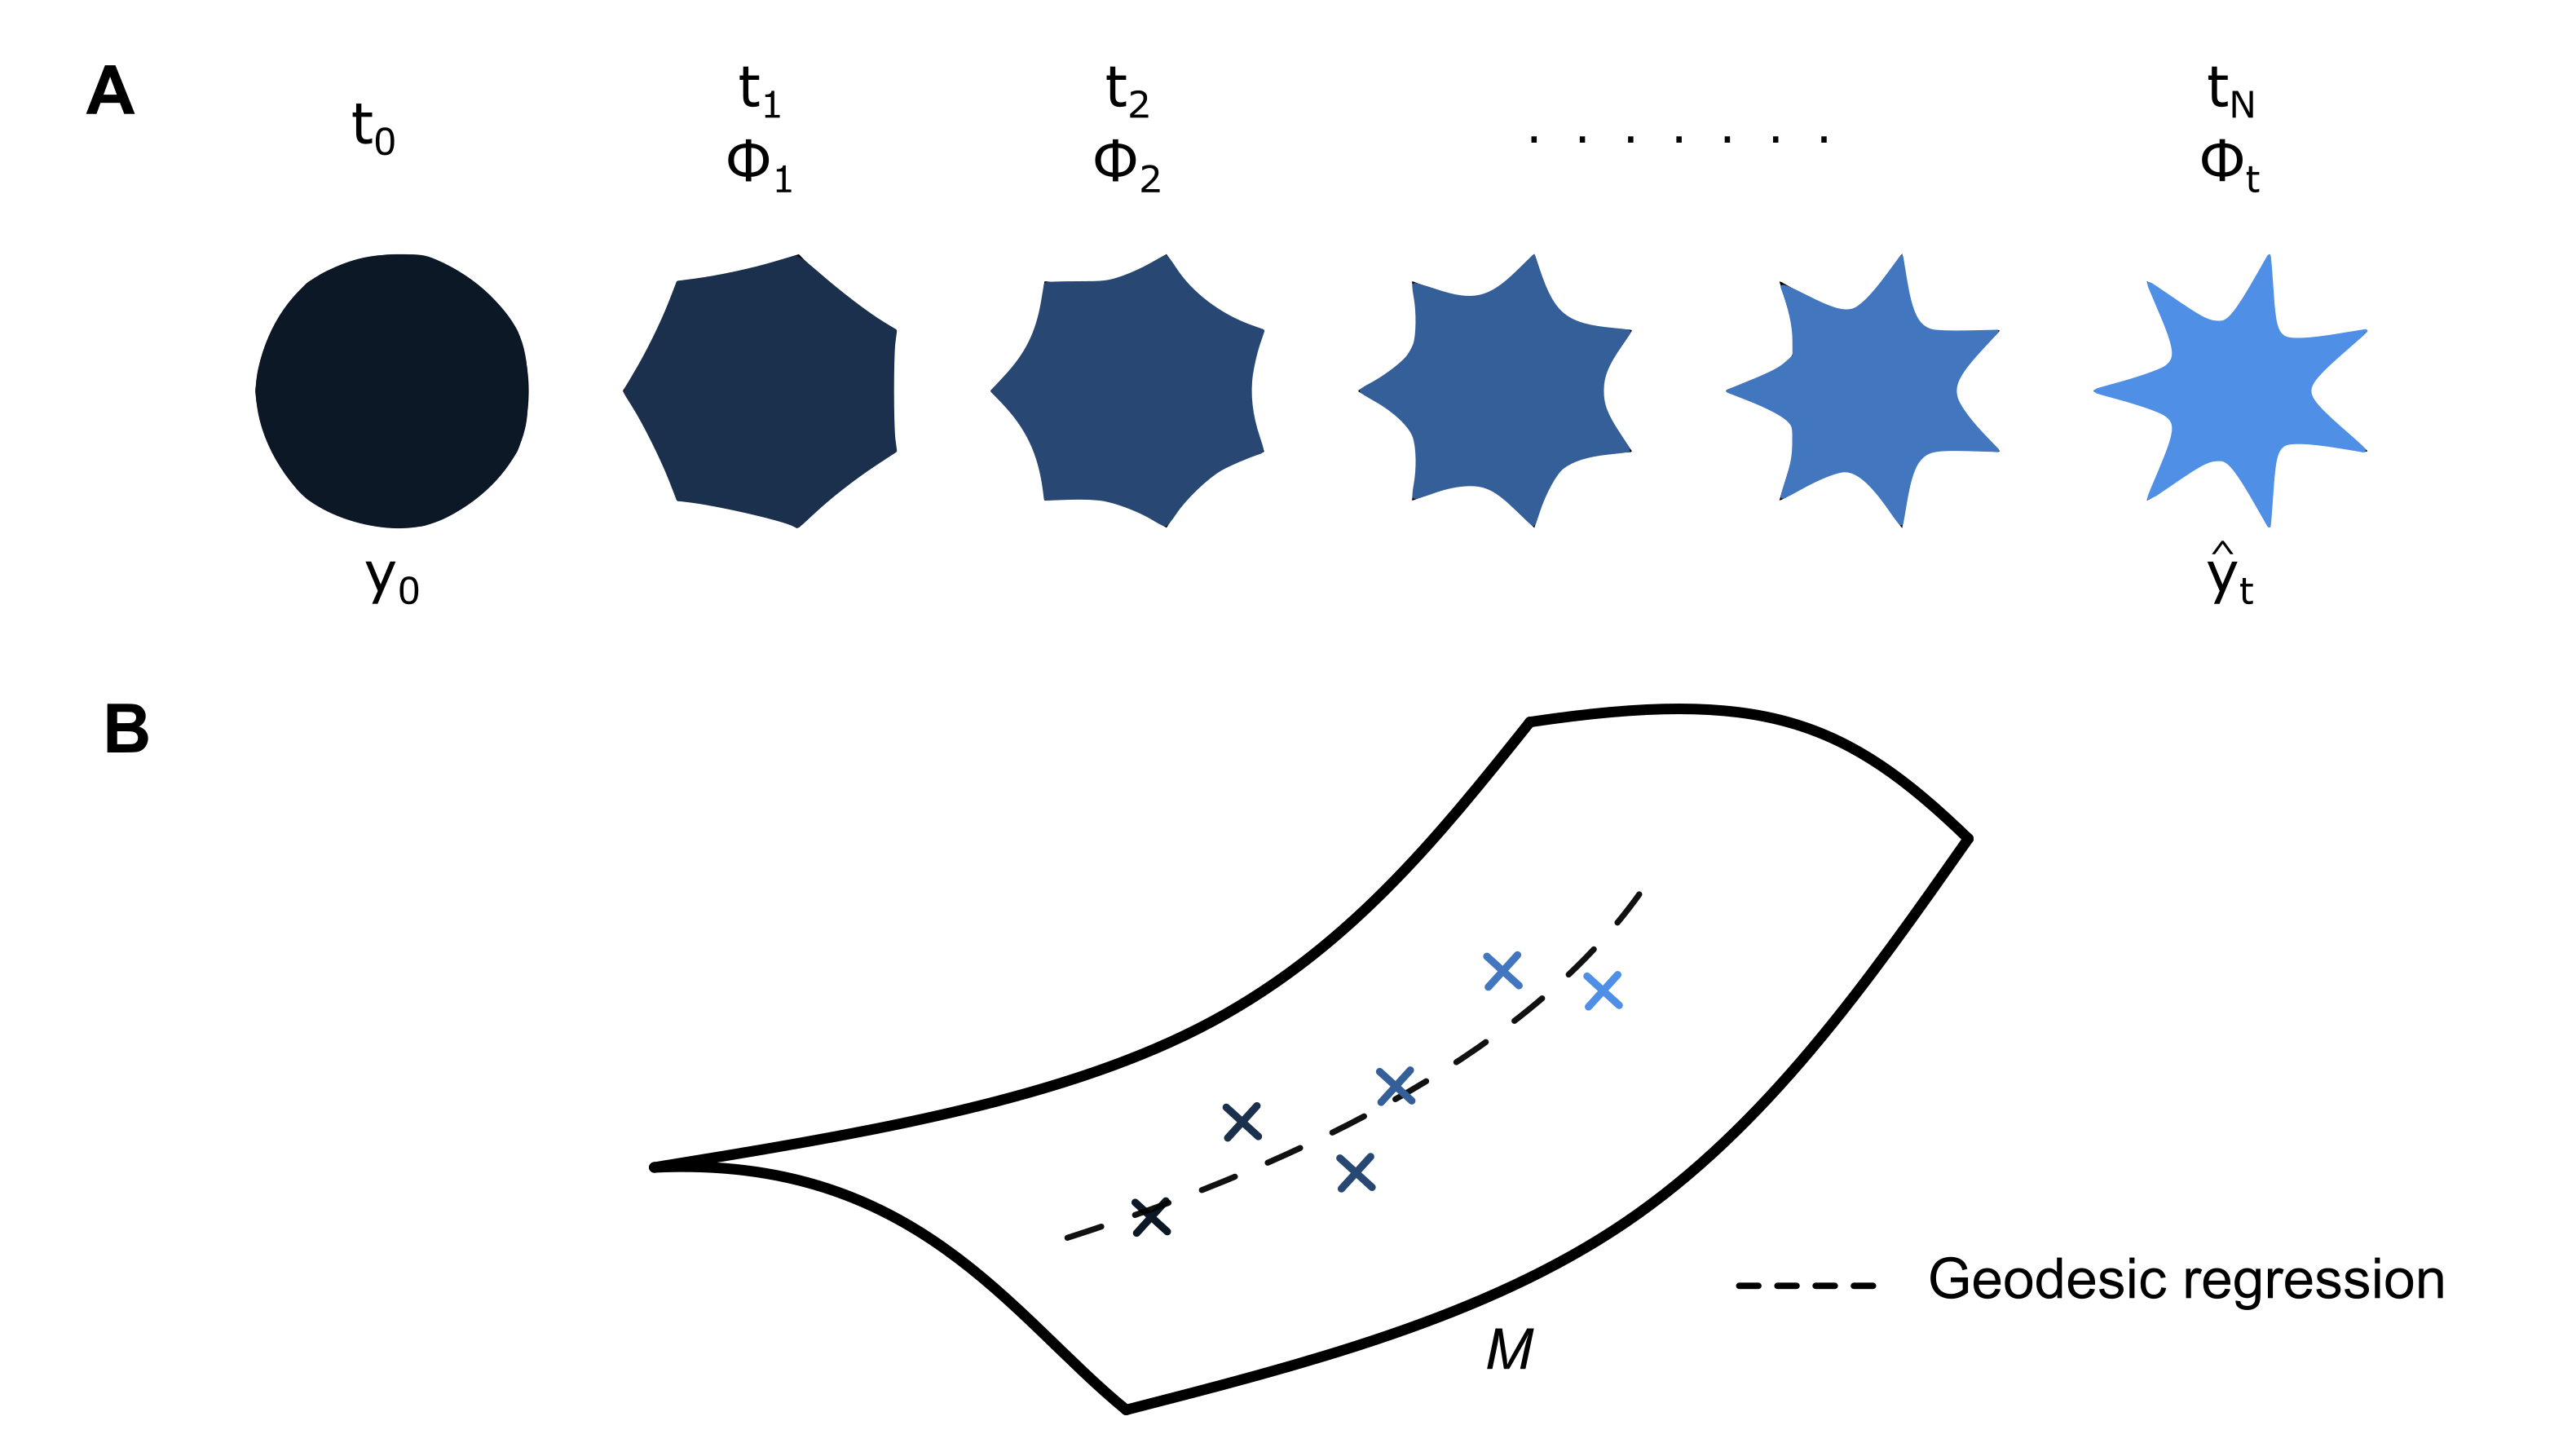
\includegraphics[scale=0.9]{fig2.png}
				\caption{\textbf{A)} Each shape in a longitudinal dataset of $N$ shapes spanning $[t_{0},t_{N}]$ can be described with a corresponding diffeomorphism at time $t$, $\phi_{t}$, acting on reference shape $y_{0}$. These diffeomorphisms are obtained from the estimation of an underlying group-average geodesic. Thus, the action of $\phi_{t}$ on $y_{0}$ leads to an estimate for the corresponding shape $\hat{y_{t}}$ \textbf{B)} Each diffeomorphism lies on a Riemannian manifold $M$, and an underlying group-average geodesic, which describes the trajectory of diffeomorphisms, can be estimated \textit{via} geodesic regression.}
				\label{fig:fig2}
			\end{figure}
	
			\subsection{Hierarchical Models} 
			
				While geodesic regression can describe an object's longitudinal trajectory over time, it is insufficient to describe the longitudinal characteristics of multiple objects in a large dataset (Figure \ref{fig:fig3}A). Thus, the LDDMM framework was further extended towards hierarchical models. Early work done by Muralidharan \textit{et al.} could estimate an underlying groupwise mean geodesic based on individual geodesics (Figure \ref{fig:fig3}B) \cite{Muralidharan2012}. They did this with a least squares estimation of the underlying mean geodesic, using Sasaki metrics to compare individual trends. This was developed further by Singh \textit{et al.} as a generalization of hierarchical linear models to a manifold-based setting \cite{Singh2015}. Schiratti \textit{et al.} took a slightly different modeling approach, wherein they first found the underlying group-average spatiotemporal trajectory and represented individual trajectories within the dataset as space and time transformations of this group-average \cite{SchirattiAllassonni2017}. This approach offers more flexibility as, unlike the former approach, it is not heavily dependent on initial time point choice, easing time reparametrization. Bône \textit{et al.} developed this approach further for shape data within the LDDMM framework specifically \cite{Bone2018, Bne2020}.

				\begin{figure}[h!]
					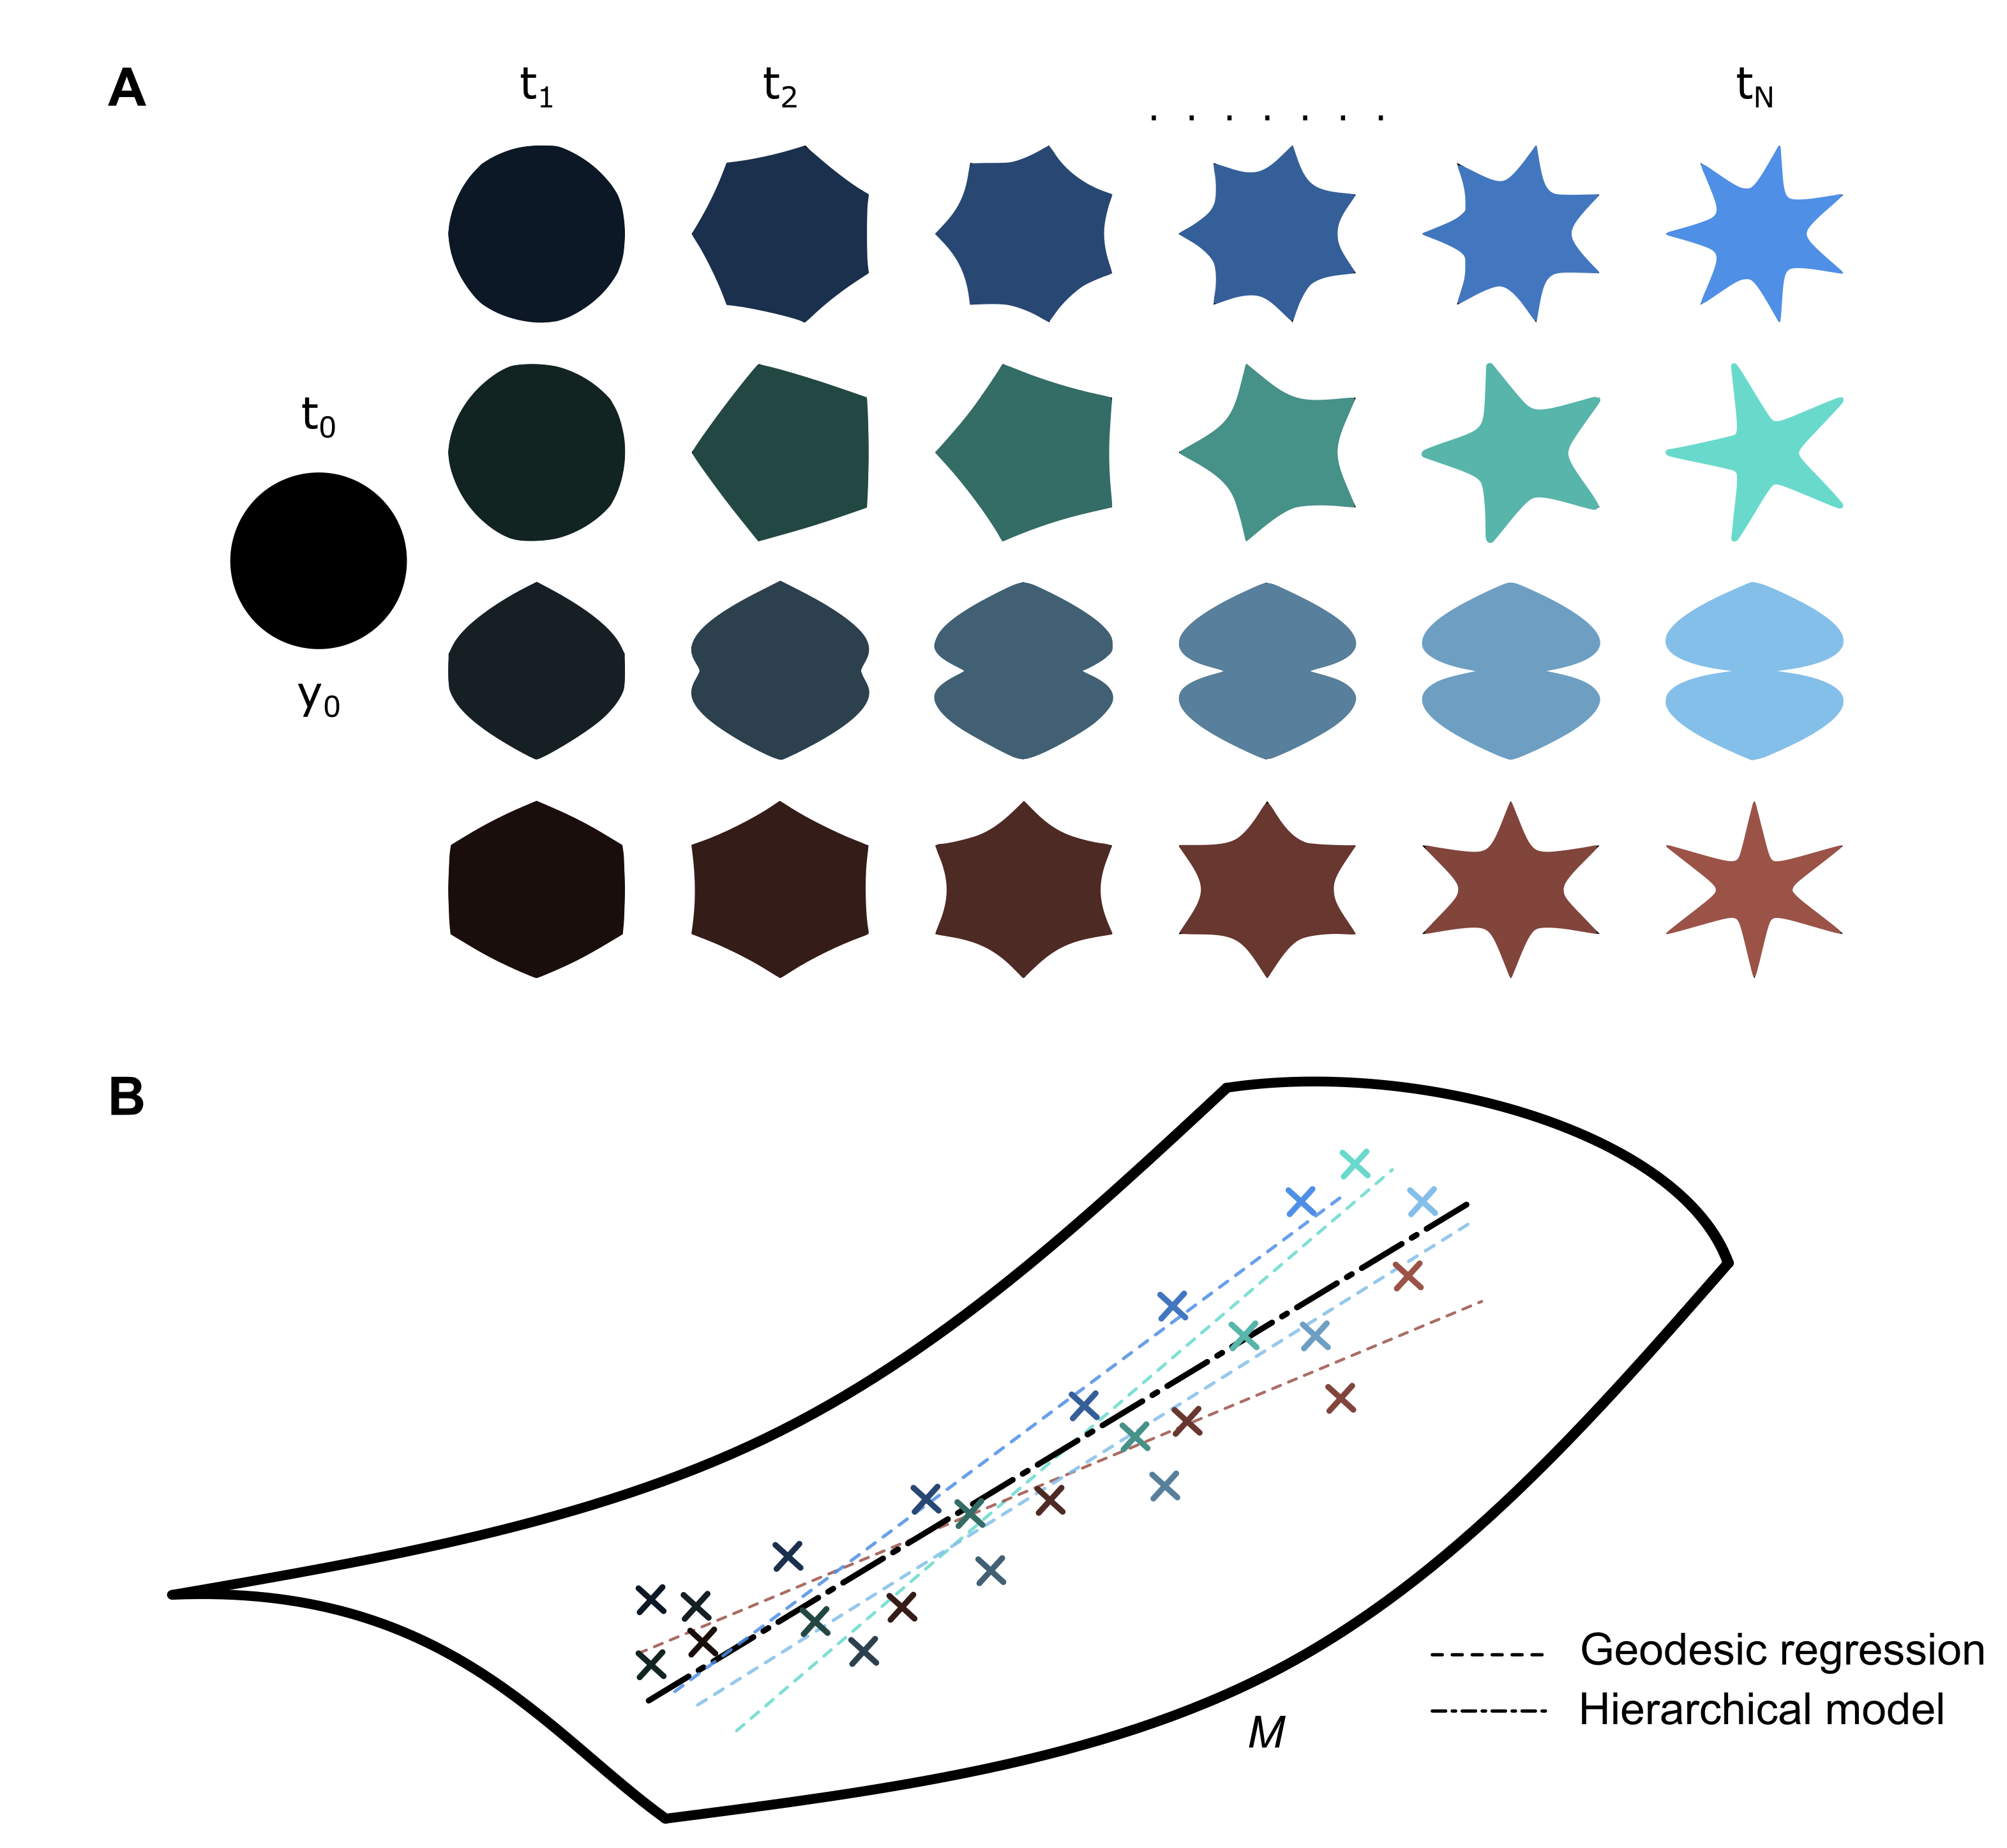
\includegraphics[scale=0.9]{fig3.png}
					\caption{\textbf{A)} A dataset of various shapes spanning $[t_{0},t_{N}]$ can be described as diffeomorphic transformations of an underlying baseline template shape $y_{0}$. \textbf{B)} Individual shape trajectories can be modeled by individual geodesic regressions, which can be used to estimate a group-average geodesic or vice-versa (\textit{i.e.}, group-average geodesic used to estimate individual trajectories). }
					\label{fig:fig3}
				\end{figure}

				Briefly, the hierarchical generative longitudinal models of Bône \textit{et al.} rely on exp-parallelization ($\text{ExpP}_{\gamma}^{v_{i}}$) and a time warp function ($\psi_{i}$) to account for individual spatial and temporal differences respectively (Equation \ref{eq:hierarchicalmodel}) \cite{Bone2018, Bne2020}. Exp-parallelization essentially offers a tool to define parallel curves on a manifold whilst retaining the underlying structure \cite{Schiratti2015, SchirattiAllassonni2017}. This enables us to define individual trajectories traversing the manifold as a variation of a group average. A time warp, on the other hand, accounts for the temporal characteristics of each individual's trajectory (\textit{i.e.}, onset time, and rate of progression).
				
%				\begin{equation}
					\begin{align}
						\text{ExpP}_{\gamma}^{v_{i}} &[\psi_{i}(t_{i,j})] \star y_{0} \mathop{\sim}\limits^{\text{iid}} \mathcal{N}_{\epsilon}(y_{i,j}, \sigma_{\epsilon}^{2})\label{eq:hierarchicalmodel} \\
						\text{where} \quad & \vert\psi_{i} : t \rightarrow \alpha_{i} \cdot (t- \tau_{i}) + t_{0} \nonumber \\ 
						& \vert v_{i} = \mathrm{Conv}(c_{0}, m_{i}), \quad m_{i} = A_{0, m_{0}^{\perp}} \cdot s_{i} \nonumber
                     \end{align}
%				\end{equation}
				
				In turn, each component of the model (Equation \ref{eq:hierarchicalmodel}) is as follows. A prediction for shape observation $j$ of subject $i$, $y_{i,j}$ is modeled as a noisy estimate with variance $\sigma_{\epsilon}^2$. $y_{i,j}$ itself is predicted as a diffeomorphic transformation of a baseline reference shape $y_{0}$ transformed by an underlying group average geodesic $\gamma$ space-shifted by exp-parallelization to match an individual's trajectory $v_{i}$. The time warp function $\psi_{i}$ accounts for temporal characteristics, where $\alpha_{i}$ denotes progression rate, $\tau_{i}$ is onset time, and $t_{0}$ is the reference time. $v_{i}$ accounts for the individuals' spatial variability and, in essence, is Equation 2 with some additional constraints. Namely, the momenta $m_{i}$ are obtained from a mixing matrix $A_{0, m_{0}^{\perp}}$ and $q$ source parameters $s_{i} = s_{i}^{(1)}, ..., s_{i}^{q}$. The parameters to be estimated which define individual trajectories are modeled as independent samples from normal distributions: 
				
%				\begin{equation}
					\begin{align}
						\alpha_{i} &\mathop{\sim}\limits^{\text{iid}} \mathcal{N}_{[0, +\infty]} (1, \sigma_{\alpha}^2) \\
						\tau_{i} &\mathop{\sim}\limits^{\text{iid}} \mathcal{N}(t_{0}, \sigma_{\tau}^2) \nonumber \\
						s_{i} &\mathop{\sim}\limits^{\text{iid}} \mathcal{N}(0, 1) \nonumber	
						\end{align}
%				\end{equation} 

				Taken together, a mixed effects model can be defined for the gathered parameters.
				Fixed effects, which account for parameters affecting the trajectories of all the subjects, can be denoted as $\theta = (\theta_{1}, \theta_{2})$. Where, $\theta_{1} = (t_{0}, \sigma_{\tau}, \sigma_{\alpha}, \sigma_{\epsilon})$ and $\theta_{2} = (y_{0}, c_{0}, m_{0}, A_{0})$. The random effects $z_{i}$ account for variations for each subject, where $z_{i} = (\alpha_{i}, \tau_{i}, s_{i})$. This nonlinear multi-parameter optimization task is computationally complex and expensive and relies on a multi-step \textit{calibration}, \textit{personalization}, and \textit{simulation} scheme detailed further in Bône \textit{et al.} \cite{Bne2020}. In brief, it utilizes a novel Monte Carlo Markov Chains-Stochastic Approximation Expectation Maximization-Gradient Descent (MCMC-SAEM-GD) algorithm detailed further in the reference. 

				\subsection{Applications and Further Works}
				
					Overall, the use of hierarchical models provides us with a structured framework to characterize longitudinal data, both on an individual and group level. The use of a group-average trajectory enables us to quantify the variation of an individual's progression from a normative scenario \cite{Kim2017}. This also has the potential for prognostic benefits. For example, Cury \textit{et al.} could detect shape changes in the thalamus of patients suffering from dementia 10 years prior to clinical symptoms by comparing healthy and diseased spatiotemporal trajectories \cite{Cury2016}. Bône \textit{et al.} have demonstrated the use of exp-parallelization and time reparametrization to transport a population average trajectory onto new subjects \cite{Bne2017}. Thus, they demonstrated that population-average normative trajectories can be leveraged to predict trends in shape change or disease progression for new, unseen subjects. Similarly, Koval \textit{et al.} implemented a manifold-based hierarchical model but in the context of graph networks \cite{Koval2018}. Specifically, they derived a population-based estimate for cortical atrophy dynamics and demonstrated the capability to characterize patient-specific atrophy dynamics. They further extended this work to account for multimodal data such as biomarker levels and cognitive impairment scores to develop a comprehensive spatiotemporal atlas of Alzheimer's disease \cite{Koval2021}. This method of integrating the use of biomarkers (\textit{i.e.,} genetic and clinical factors) alongside imaging has gained traction and not only demonstrates soundness in and of itself \cite{Dalca2015} but also has the potential to enhance the predictive capacity of existing frameworks with multimodality. Couronne \textit{et al.} further demonstrated the efficacy of multimodal models in the context of Parkinson's disease prognosis \cite{Couronne2019}. Utilizing both imaging and neurophysiological test score data, they demonstrated the robustness and efficacy of multimodality to improve predictive performance.
					
					Nevertheless, the hierarchical model framework is still being developed further to refine its modeling efficacy and integrate newer technological developments. As opposed to modeling correlations along a manifold as quasi-linear in the manner of geodesics, Hanik \textit{et al.} proposed to utilize generalized Bézier curves to model nonlinear relationships with the rationale that many biological processes are nonlinear (\textit{e.g.,} cardiac motion) \cite{Hanik2022}. Their initial work demonstrated the potential for extending this principle further and potentially decomposing longitudinal trends (\textit{i.e.,} disease progression) into different components of a nonlinear curve, enabling more granular analyses. Hong \textit{et al.} also investigated the effects of subject-specific characteristics by including multivariate intercept models in their formulation of a hierarchical geodesic model \cite{Hong2019}. Debavelaere \textit{et al.} developed a methodology to investigate datasets with heterogeneous populations (\textit{i.e.,} a dataset with diverging longitudinal dynamics) \cite{Debavelaere2020}. They developed an unsupervised algorithm that is able to detect clusters of subgroups within a dataset and differentiate their trajectories, accounting for diverging or converging trajectories from a population normal. Furthermore, the advent of DL has led to augmentations of the LDDMM framework due to its increased computational efficiency of processing large datasets\cite{Yang2023, BenAmor2022}. Bône \textit{et al.} demonstrated the use of autoencoders to learn an atlas and class of diffeomorphisms that describe a dataset of shapes and meshes \cite{Bne2019}. They further extended their work to also account for the texture (\textit{i.e.,} appearance) of images \cite{Bne2020a}. Pathan and Hong also demonstrated the potential of using DL to learn vector momenta utilized in the LDDMM framework \cite{pathan2018}. Other novel developments include the utilization of implicit neural representations (INRs) \cite{NEURIPS2020_53c04118}. Dummer \textit{et al.} demonstrated the potential of using INRs to extend the LDDMM framework towards increased robustness and resolution independence \cite{dummer2023}. 
				
					To surmise, the LDDMM framework is a powerful tool for representing and modeling a dataset of shapes. Assuming an underlying template shape, the LDDMM framework represents individual shapes as diffeomorphic transformations of this template. These diffeomorphisms lie on an infinite dimensional Riemannian manifold, thus relying on geodesic regression and parallel transport tools to estimate the longitudinal trajectories traversing the underlying data manifold. Hierarchical models can then be utilized to model differing spatiotemporal trajectories of a population, capable of estimating population average spatiotemporal trajectories and also quantifying intra and inter-individual differences. Whilst, in recent years, the proliferation of DL-based techniques has seemingly eclipsed LDDMM-based techniques, the framework is continuously developing. In fact, many of the developments seek to utilize DL tools to accelerate the framework and increase its efficacy. LDDMM methods are readily available in several software packages and applications such as Deformetrica \cite{Bne2018}, Leaspy (https://leaspy.readthedocs.io/en/stable/), and Morphomatics \cite{Morphomatics}.  
					